\documentclass[11pt]{article}
\usepackage[textwidth=18.0cm, textheight=23.0cm, top=2.0cm]{geometry}
\usepackage{pst-all}
\usepackage{amssymb}
\usepackage{tikz}
\usepackage{underscore}\begin{document}
\pagestyle{empty}


ClassName: \underline{\textbf{Class_03.2bp-31}}
\par
BinSize: \underline{\textbf{40 × 40}}
\par
ReduceSize: \underline{\textbf{40 × 40}}
\par
TypeNum: \underline{\textbf{76}}
\par
Num: \underline{\textbf{80}}
\par
OutS: \underline{\textbf{28800}}
\par
InS: \underline{\textbf{25445}}
\par
Rate: \underline{\textbf{0.884}}
\par
UB: \underline{\textbf{18}}
\par
LB0: \underline{\textbf{18}}
\par
LB: \underline{\textbf{18}}
\par
LBWithCut: \underline{\textbf{18}}
\par
NodeCut: \underline{\textbf{0}}
\par
ExtendedNodeCnt: \underline{\textbf{1}}
\par
GenNodeCnt: \underline{\textbf{1}}
\par
PrimalNode: \underline{\textbf{0}}
\par
ColumnCount: \underline{\textbf{18}}
\par
TotalCutCount: \underline{\textbf{0}}
\par
RootCutCount: \underline{\textbf{0}}
\par
LPSolverCnt: \underline{\textbf{1}}
\par
PricingSolverCnt: \underline{\textbf{0}}
\par
BranchAndBoundNum: \underline{\textbf{1}}
\par
isOpt: \underline{\textbf{true}}
\par
TimeOnInitSolution: \underline{\textbf{0.170 s}}
\par
TimeOnPrimal: \underline{\textbf{0.000 s}}
\par
TimeOnPricing: \underline{\textbf{0.000 s}}
\par
TimeOnRmp: \underline{\textbf{0.109 s}}
\par
TotalTime: \underline{\textbf{0.341 s}}
\par
\newpage


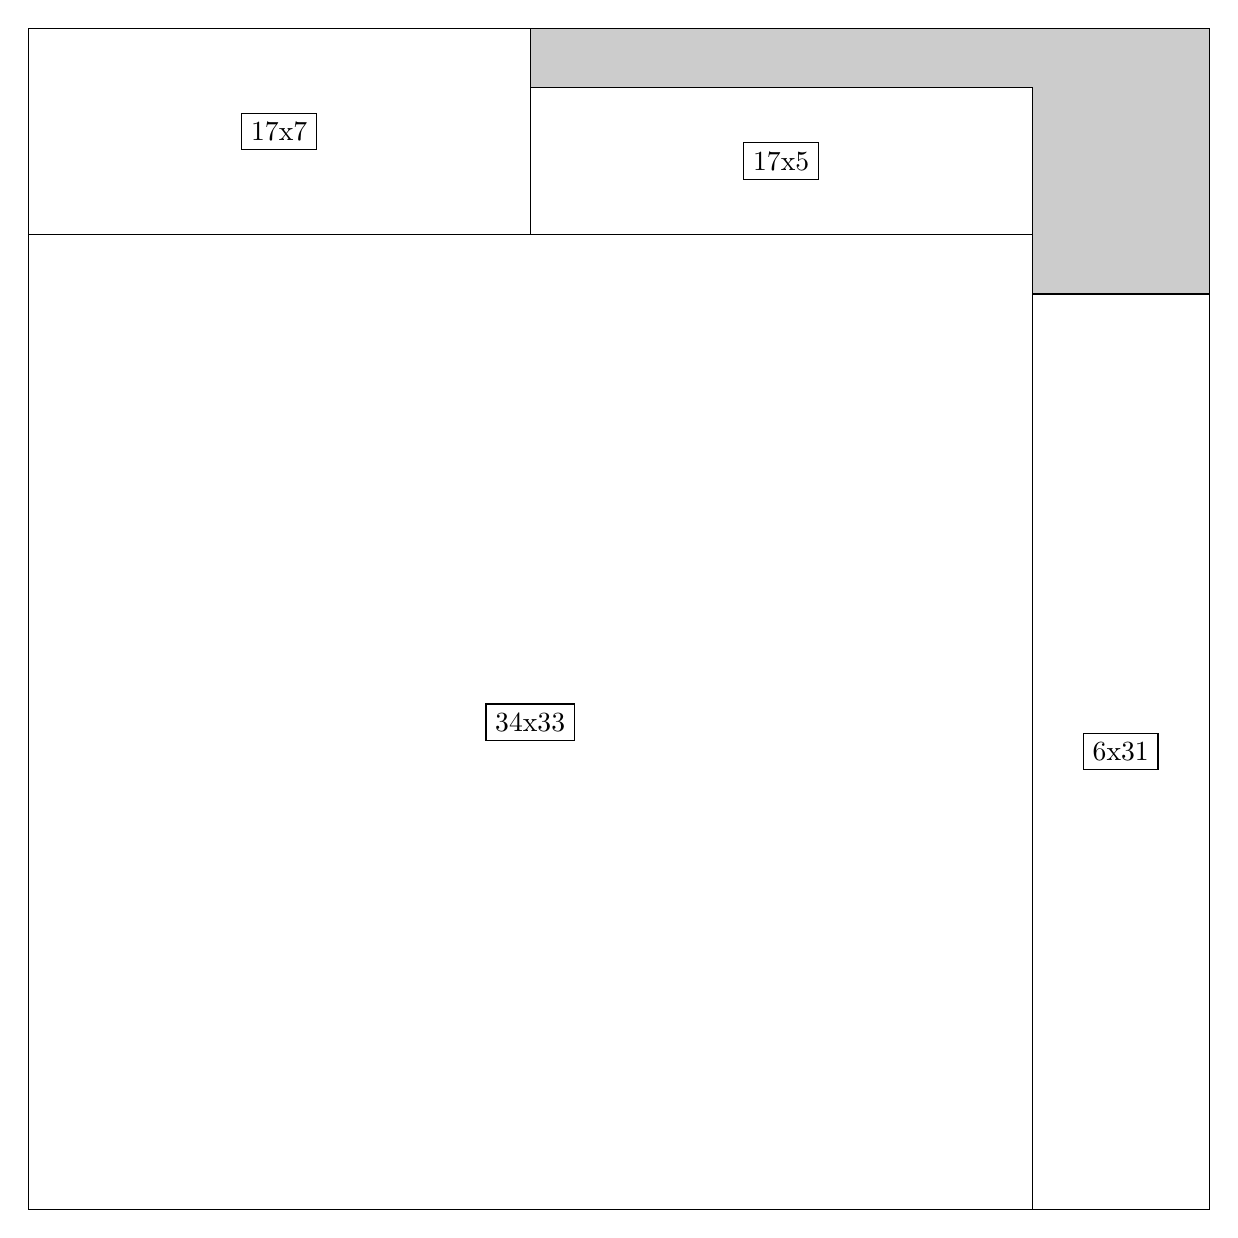
\begin{tikzpicture}[shorten >=1pt,scale=1.0,every node/.style={scale=1.0},->]
\tikzstyle{vertex}=[circle,fill=black!25,minimum size=14pt,inner sep=0pt]
\filldraw[fill=gray!40!white, draw=black] (0,0) rectangle (15.0,15.0);
\foreach \name/\x/\y/\w/\h in {34x33/0.0/0.0/12.75/12.375,6x31/12.75/0.0/2.25/11.625,17x7/0.0/12.375/6.375/2.625,17x5/6.375/12.375/6.375/1.875}
\filldraw[fill=white!40!white, draw=black] (\x,\y) rectangle node[draw] (\name) {\name} ++(\w,\h);
\end{tikzpicture}


w =34 , h =33 , x =0 , y =0 , v =1122
\par
w =6 , h =31 , x =34 , y =0 , v =186
\par
w =17 , h =7 , x =0 , y =33 , v =119
\par
w =17 , h =5 , x =17 , y =33 , v =85
\par
\newpage


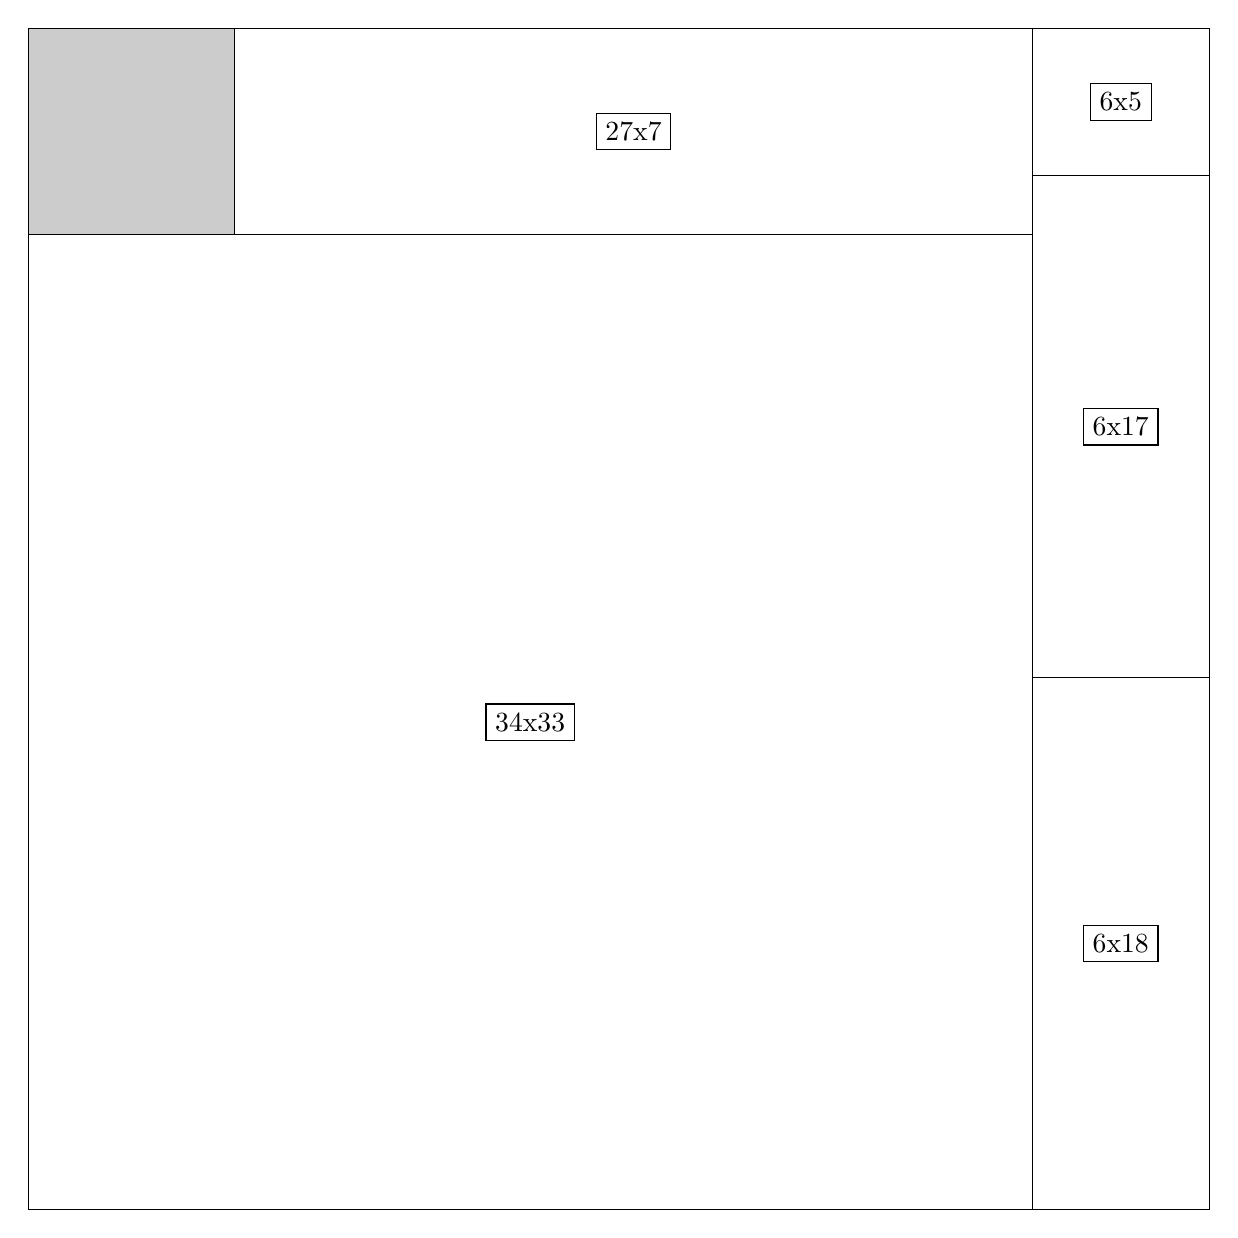
\begin{tikzpicture}[shorten >=1pt,scale=1.0,every node/.style={scale=1.0},->]
\tikzstyle{vertex}=[circle,fill=black!25,minimum size=14pt,inner sep=0pt]
\filldraw[fill=gray!40!white, draw=black] (0,0) rectangle (15.0,15.0);
\foreach \name/\x/\y/\w/\h in {34x33/0.0/0.0/12.75/12.375,27x7/2.625/12.375/10.125/2.625,6x18/12.75/0.0/2.25/6.75,6x17/12.75/6.75/2.25/6.375,6x5/12.75/13.125/2.25/1.875}
\filldraw[fill=white!40!white, draw=black] (\x,\y) rectangle node[draw] (\name) {\name} ++(\w,\h);
\end{tikzpicture}


w =34 , h =33 , x =0 , y =0 , v =1122
\par
w =27 , h =7 , x =7 , y =33 , v =189
\par
w =6 , h =18 , x =34 , y =0 , v =108
\par
w =6 , h =17 , x =34 , y =18 , v =102
\par
w =6 , h =5 , x =34 , y =35 , v =30
\par
\newpage


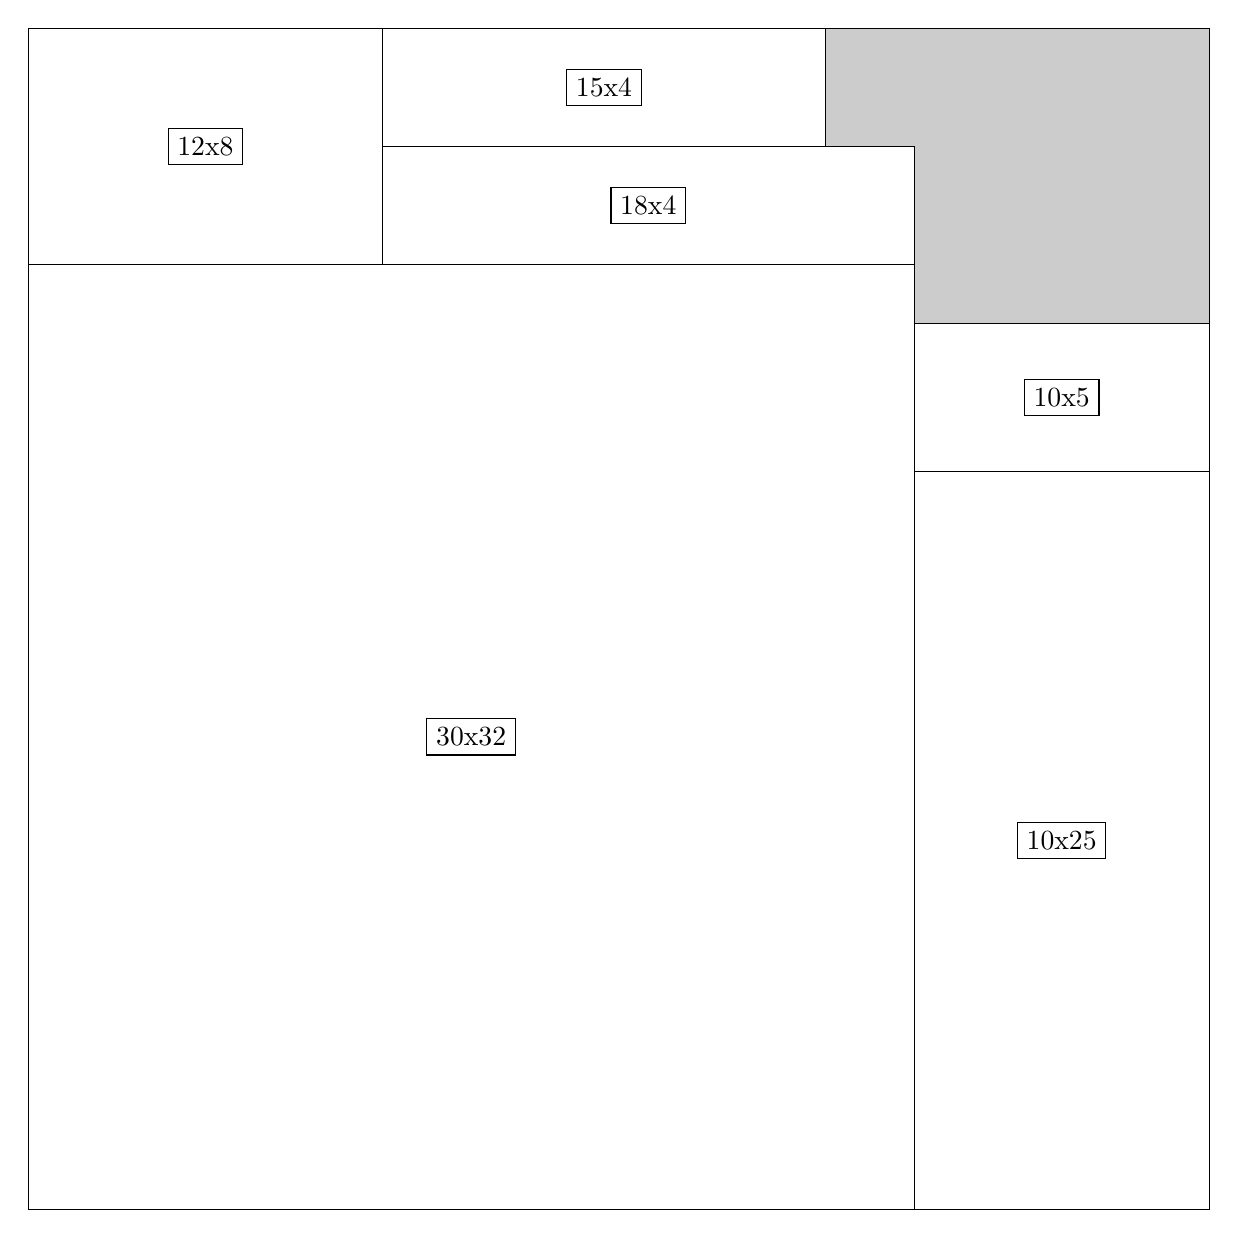
\begin{tikzpicture}[shorten >=1pt,scale=1.0,every node/.style={scale=1.0},->]
\tikzstyle{vertex}=[circle,fill=black!25,minimum size=14pt,inner sep=0pt]
\filldraw[fill=gray!40!white, draw=black] (0,0) rectangle (15.0,15.0);
\foreach \name/\x/\y/\w/\h in {10x25/11.25/0.0/3.75/9.375,30x32/0.0/0.0/11.25/12.0,12x8/0.0/12.0/4.5/3.0,18x4/4.5/12.0/6.75/1.5,15x4/4.5/13.5/5.625/1.5,10x5/11.25/9.375/3.75/1.875}
\filldraw[fill=white!40!white, draw=black] (\x,\y) rectangle node[draw] (\name) {\name} ++(\w,\h);
\end{tikzpicture}


w =10 , h =25 , x =30 , y =0 , v =250
\par
w =30 , h =32 , x =0 , y =0 , v =960
\par
w =12 , h =8 , x =0 , y =32 , v =96
\par
w =18 , h =4 , x =12 , y =32 , v =72
\par
w =15 , h =4 , x =12 , y =36 , v =60
\par
w =10 , h =5 , x =30 , y =25 , v =50
\par
\newpage


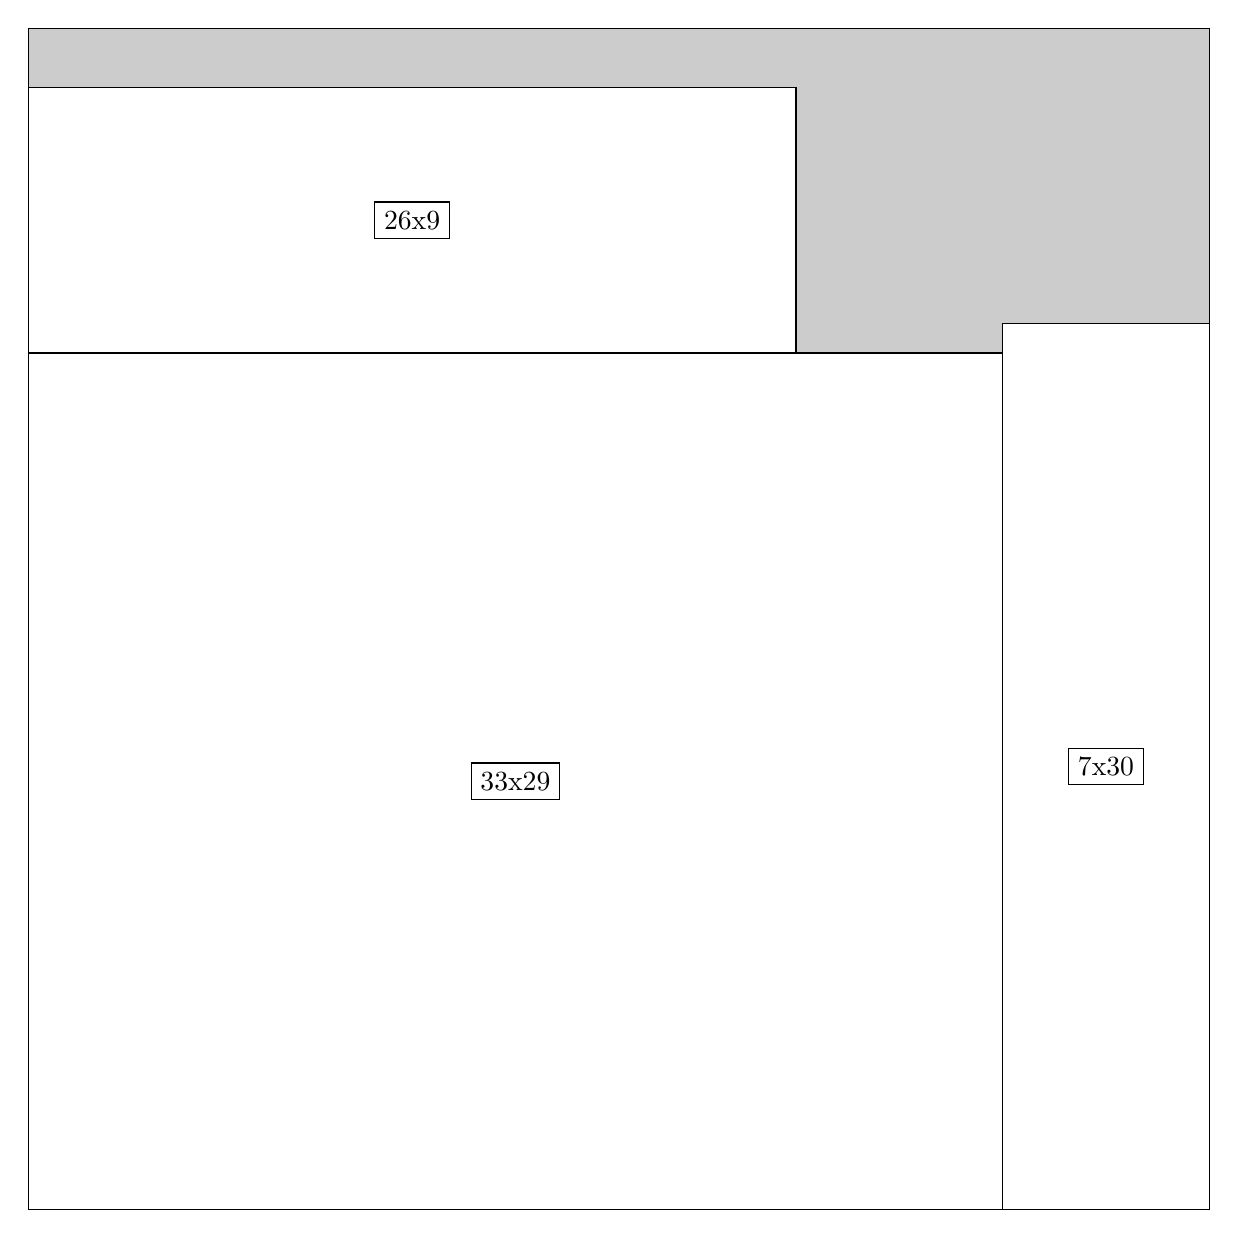
\begin{tikzpicture}[shorten >=1pt,scale=1.0,every node/.style={scale=1.0},->]
\tikzstyle{vertex}=[circle,fill=black!25,minimum size=14pt,inner sep=0pt]
\filldraw[fill=gray!40!white, draw=black] (0,0) rectangle (15.0,15.0);
\foreach \name/\x/\y/\w/\h in {33x29/0.0/0.0/12.375/10.875,26x9/0.0/10.875/9.75/3.375,7x30/12.375/0.0/2.625/11.25}
\filldraw[fill=white!40!white, draw=black] (\x,\y) rectangle node[draw] (\name) {\name} ++(\w,\h);
\end{tikzpicture}


w =33 , h =29 , x =0 , y =0 , v =957
\par
w =26 , h =9 , x =0 , y =29 , v =234
\par
w =7 , h =30 , x =33 , y =0 , v =210
\par
\newpage


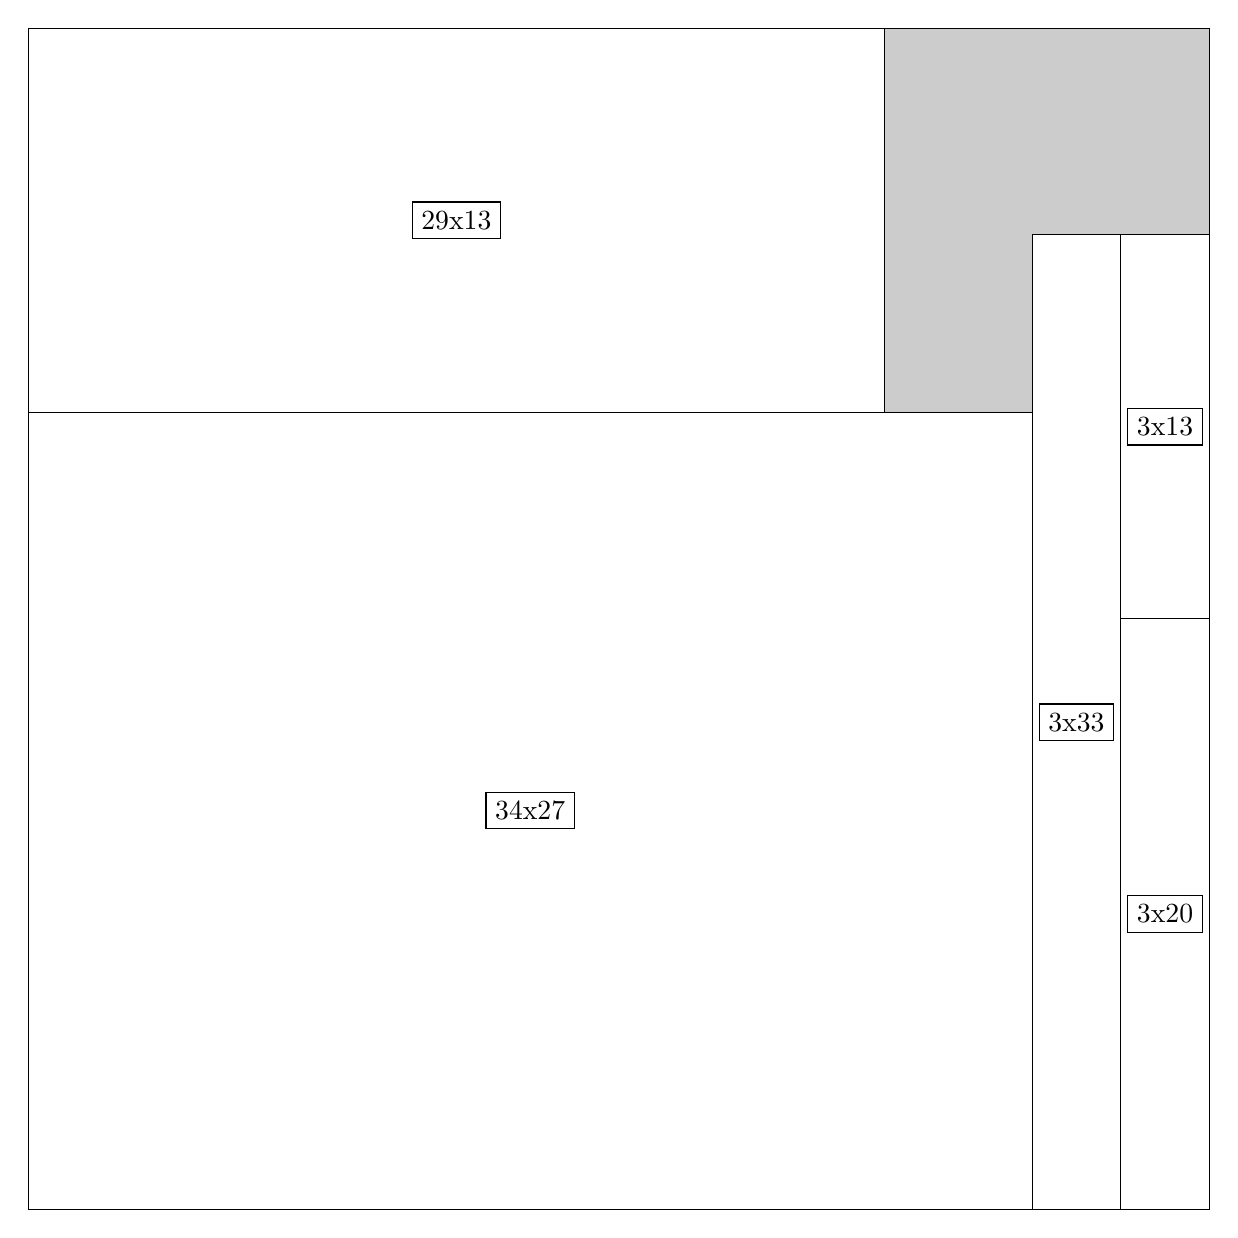
\begin{tikzpicture}[shorten >=1pt,scale=1.0,every node/.style={scale=1.0},->]
\tikzstyle{vertex}=[circle,fill=black!25,minimum size=14pt,inner sep=0pt]
\filldraw[fill=gray!40!white, draw=black] (0,0) rectangle (15.0,15.0);
\foreach \name/\x/\y/\w/\h in {34x27/0.0/0.0/12.75/10.125,29x13/0.0/10.125/10.875/4.875,3x33/12.75/0.0/1.125/12.375,3x20/13.875/0.0/1.125/7.5,3x13/13.875/7.5/1.125/4.875}
\filldraw[fill=white!40!white, draw=black] (\x,\y) rectangle node[draw] (\name) {\name} ++(\w,\h);
\end{tikzpicture}


w =34 , h =27 , x =0 , y =0 , v =918
\par
w =29 , h =13 , x =0 , y =27 , v =377
\par
w =3 , h =33 , x =34 , y =0 , v =99
\par
w =3 , h =20 , x =37 , y =0 , v =60
\par
w =3 , h =13 , x =37 , y =20 , v =39
\par
\newpage


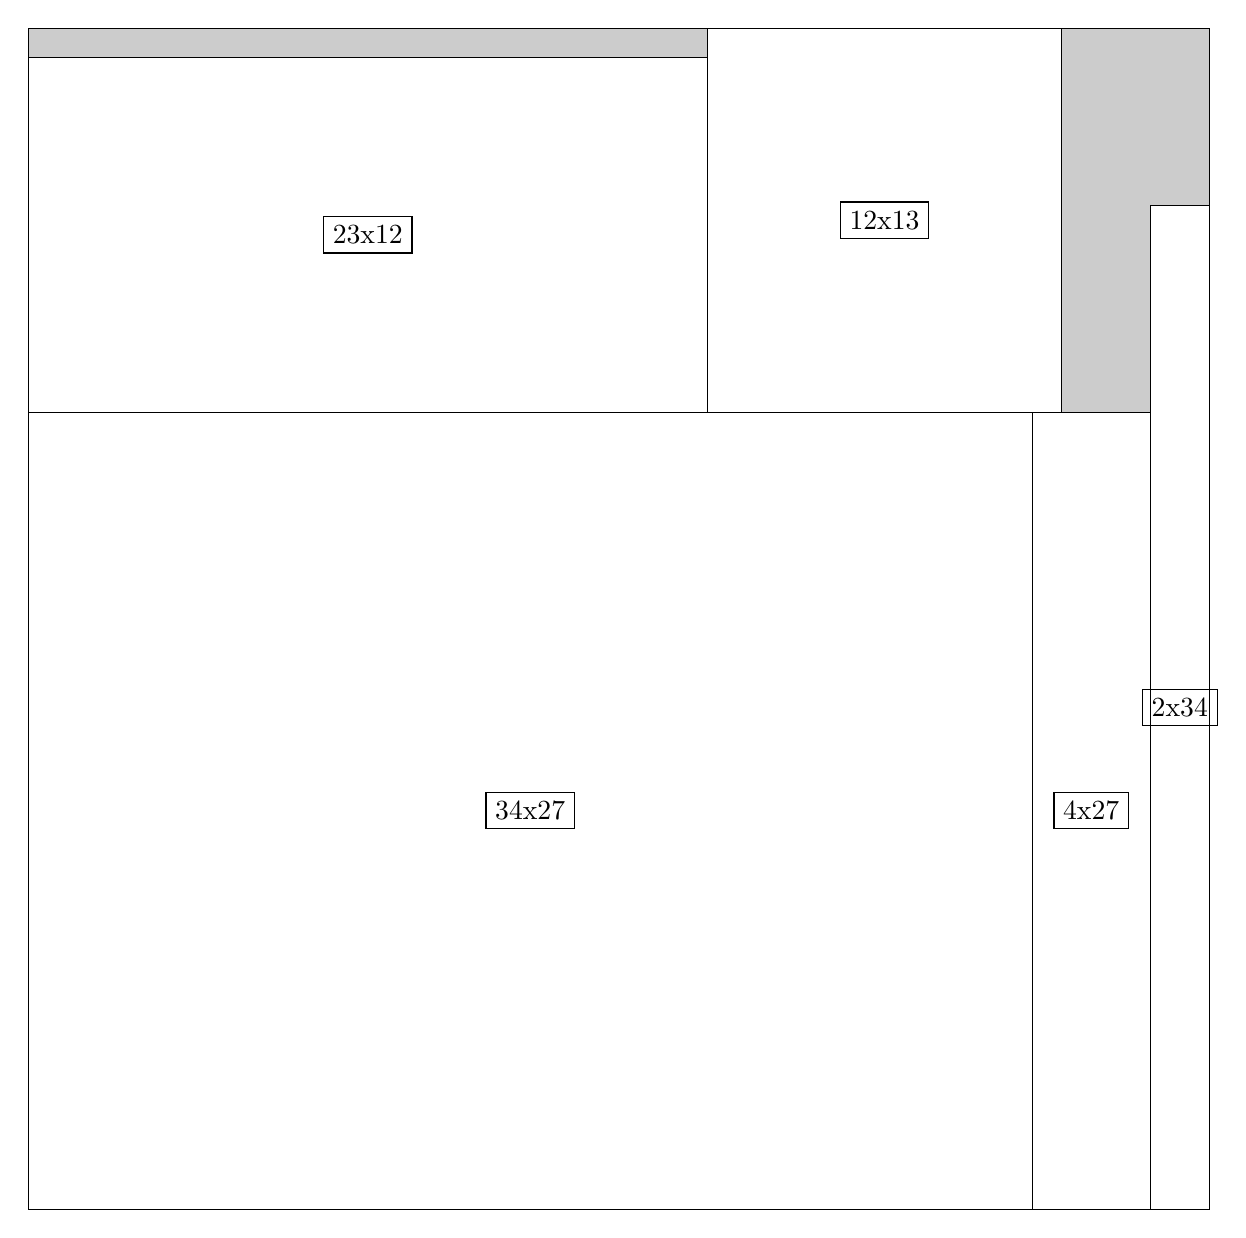
\begin{tikzpicture}[shorten >=1pt,scale=1.0,every node/.style={scale=1.0},->]
\tikzstyle{vertex}=[circle,fill=black!25,minimum size=14pt,inner sep=0pt]
\filldraw[fill=gray!40!white, draw=black] (0,0) rectangle (15.0,15.0);
\foreach \name/\x/\y/\w/\h in {34x27/0.0/0.0/12.75/10.125,23x12/0.0/10.125/8.625/4.5,12x13/8.625/10.125/4.5/4.875,4x27/12.75/0.0/1.5/10.125,2x34/14.25/0.0/0.75/12.75}
\filldraw[fill=white!40!white, draw=black] (\x,\y) rectangle node[draw] (\name) {\name} ++(\w,\h);
\end{tikzpicture}


w =34 , h =27 , x =0 , y =0 , v =918
\par
w =23 , h =12 , x =0 , y =27 , v =276
\par
w =12 , h =13 , x =23 , y =27 , v =156
\par
w =4 , h =27 , x =34 , y =0 , v =108
\par
w =2 , h =34 , x =38 , y =0 , v =68
\par
\newpage


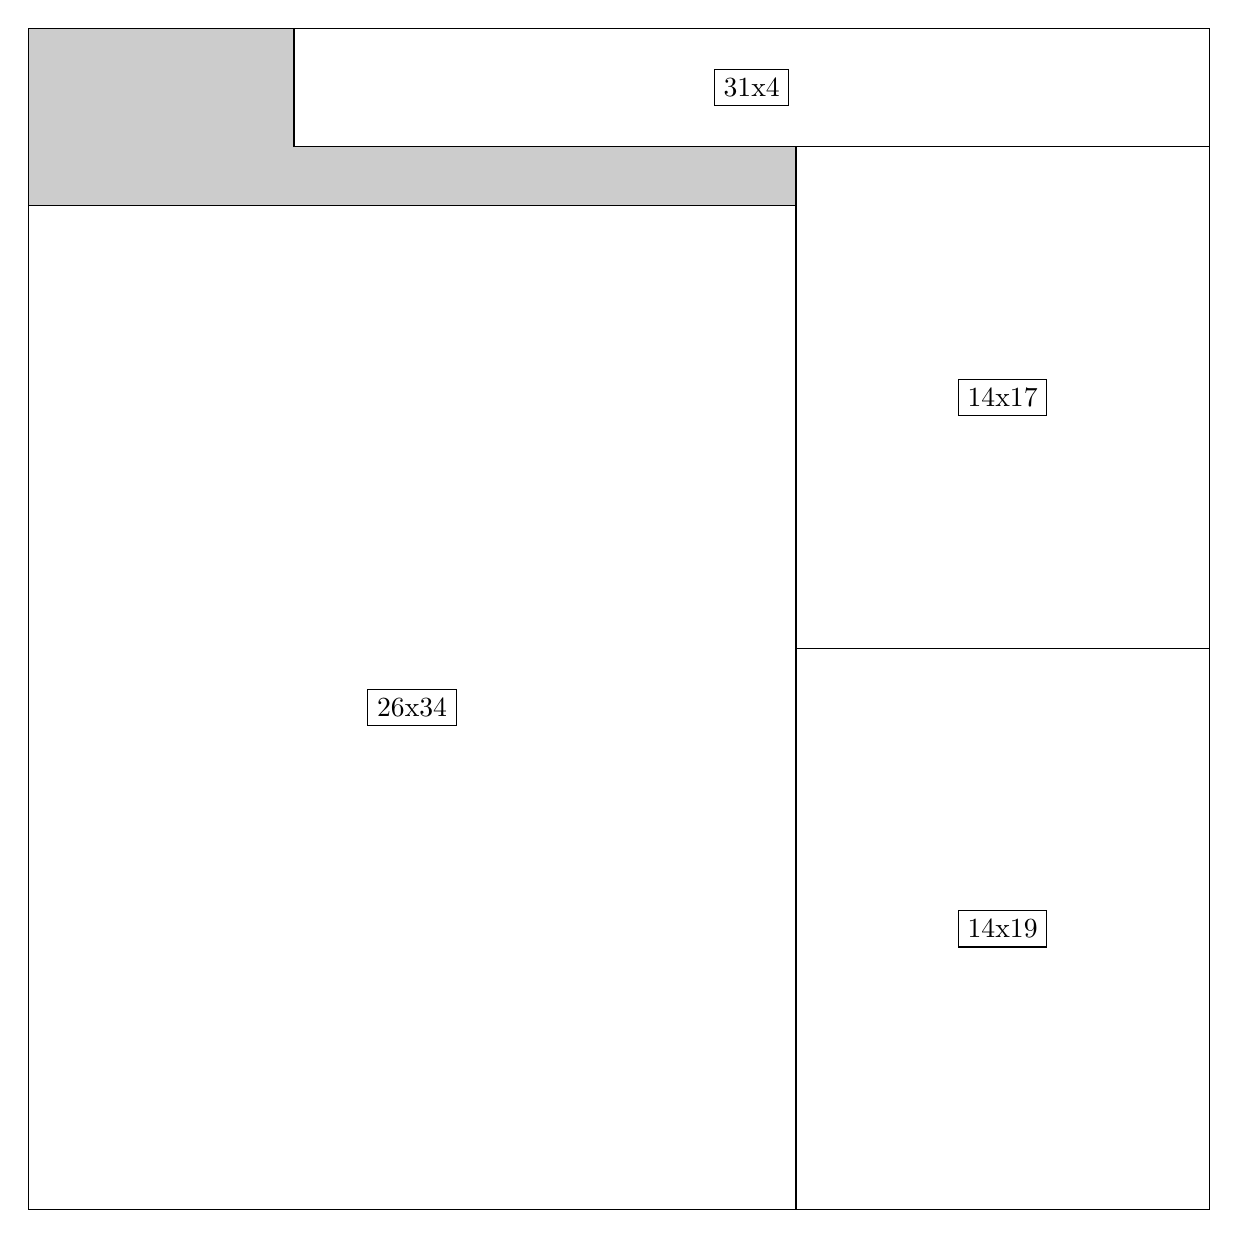
\begin{tikzpicture}[shorten >=1pt,scale=1.0,every node/.style={scale=1.0},->]
\tikzstyle{vertex}=[circle,fill=black!25,minimum size=14pt,inner sep=0pt]
\filldraw[fill=gray!40!white, draw=black] (0,0) rectangle (15.0,15.0);
\foreach \name/\x/\y/\w/\h in {26x34/0.0/0.0/9.75/12.75,14x19/9.75/0.0/5.25/7.125,14x17/9.75/7.125/5.25/6.375,31x4/3.375/13.5/11.625/1.5}
\filldraw[fill=white!40!white, draw=black] (\x,\y) rectangle node[draw] (\name) {\name} ++(\w,\h);
\end{tikzpicture}


w =26 , h =34 , x =0 , y =0 , v =884
\par
w =14 , h =19 , x =26 , y =0 , v =266
\par
w =14 , h =17 , x =26 , y =19 , v =238
\par
w =31 , h =4 , x =9 , y =36 , v =124
\par
\newpage


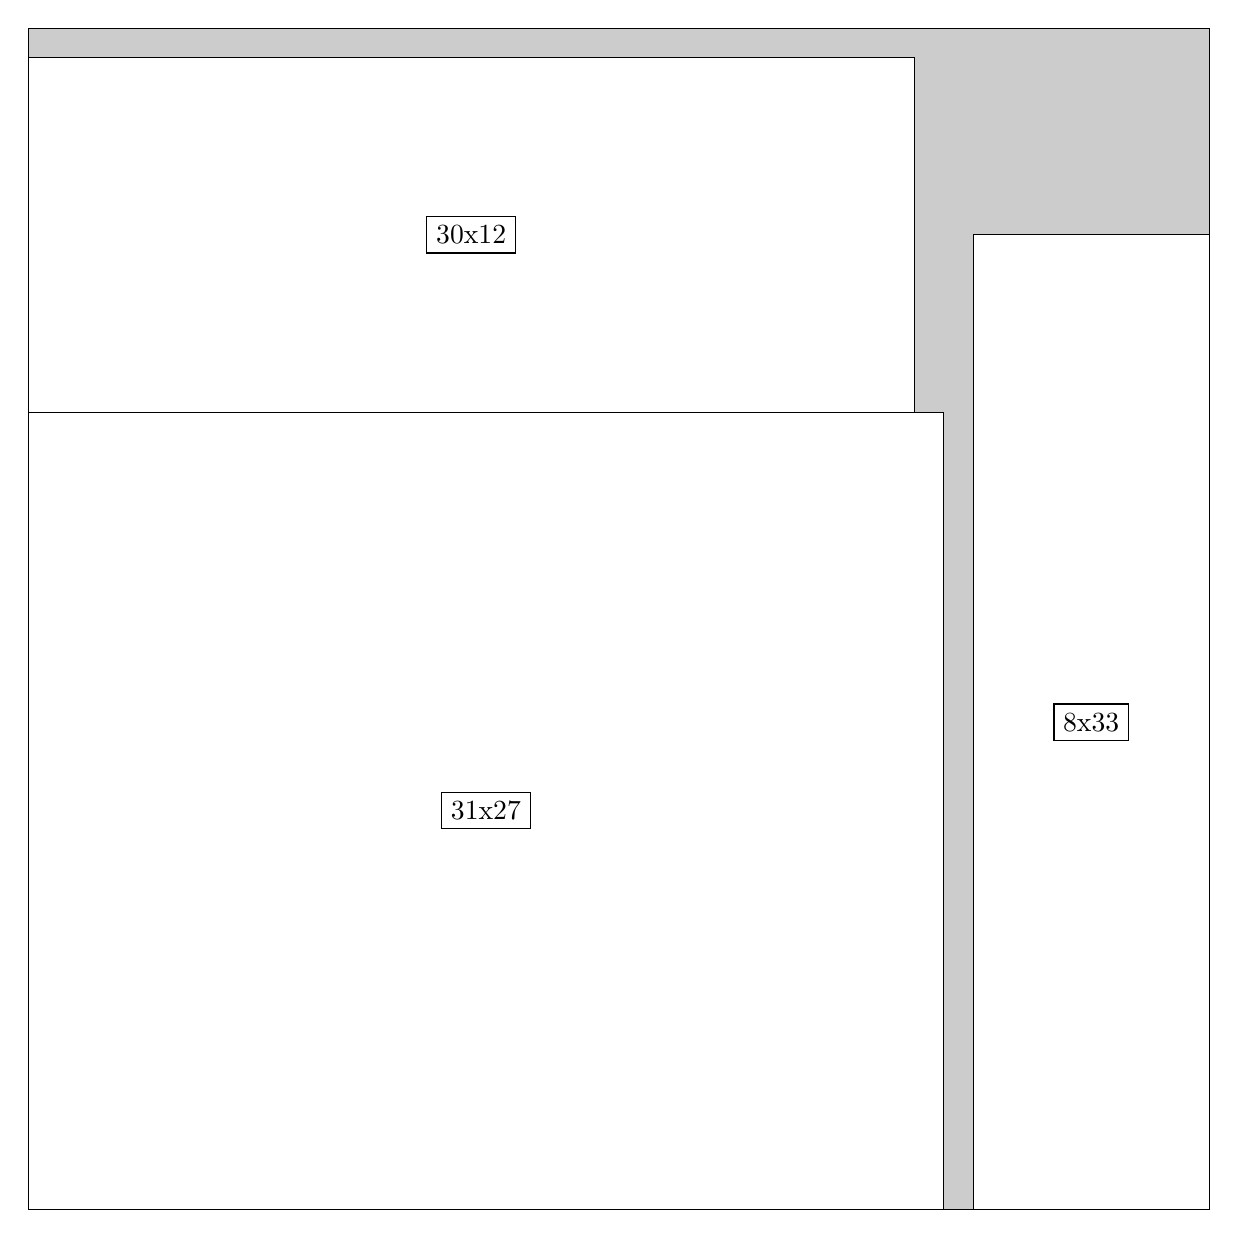
\begin{tikzpicture}[shorten >=1pt,scale=1.0,every node/.style={scale=1.0},->]
\tikzstyle{vertex}=[circle,fill=black!25,minimum size=14pt,inner sep=0pt]
\filldraw[fill=gray!40!white, draw=black] (0,0) rectangle (15.0,15.0);
\foreach \name/\x/\y/\w/\h in {31x27/0.0/0.0/11.625/10.125,30x12/0.0/10.125/11.25/4.5,8x33/12.0/0.0/3.0/12.375}
\filldraw[fill=white!40!white, draw=black] (\x,\y) rectangle node[draw] (\name) {\name} ++(\w,\h);
\end{tikzpicture}


w =31 , h =27 , x =0 , y =0 , v =837
\par
w =30 , h =12 , x =0 , y =27 , v =360
\par
w =8 , h =33 , x =32 , y =0 , v =264
\par
\newpage


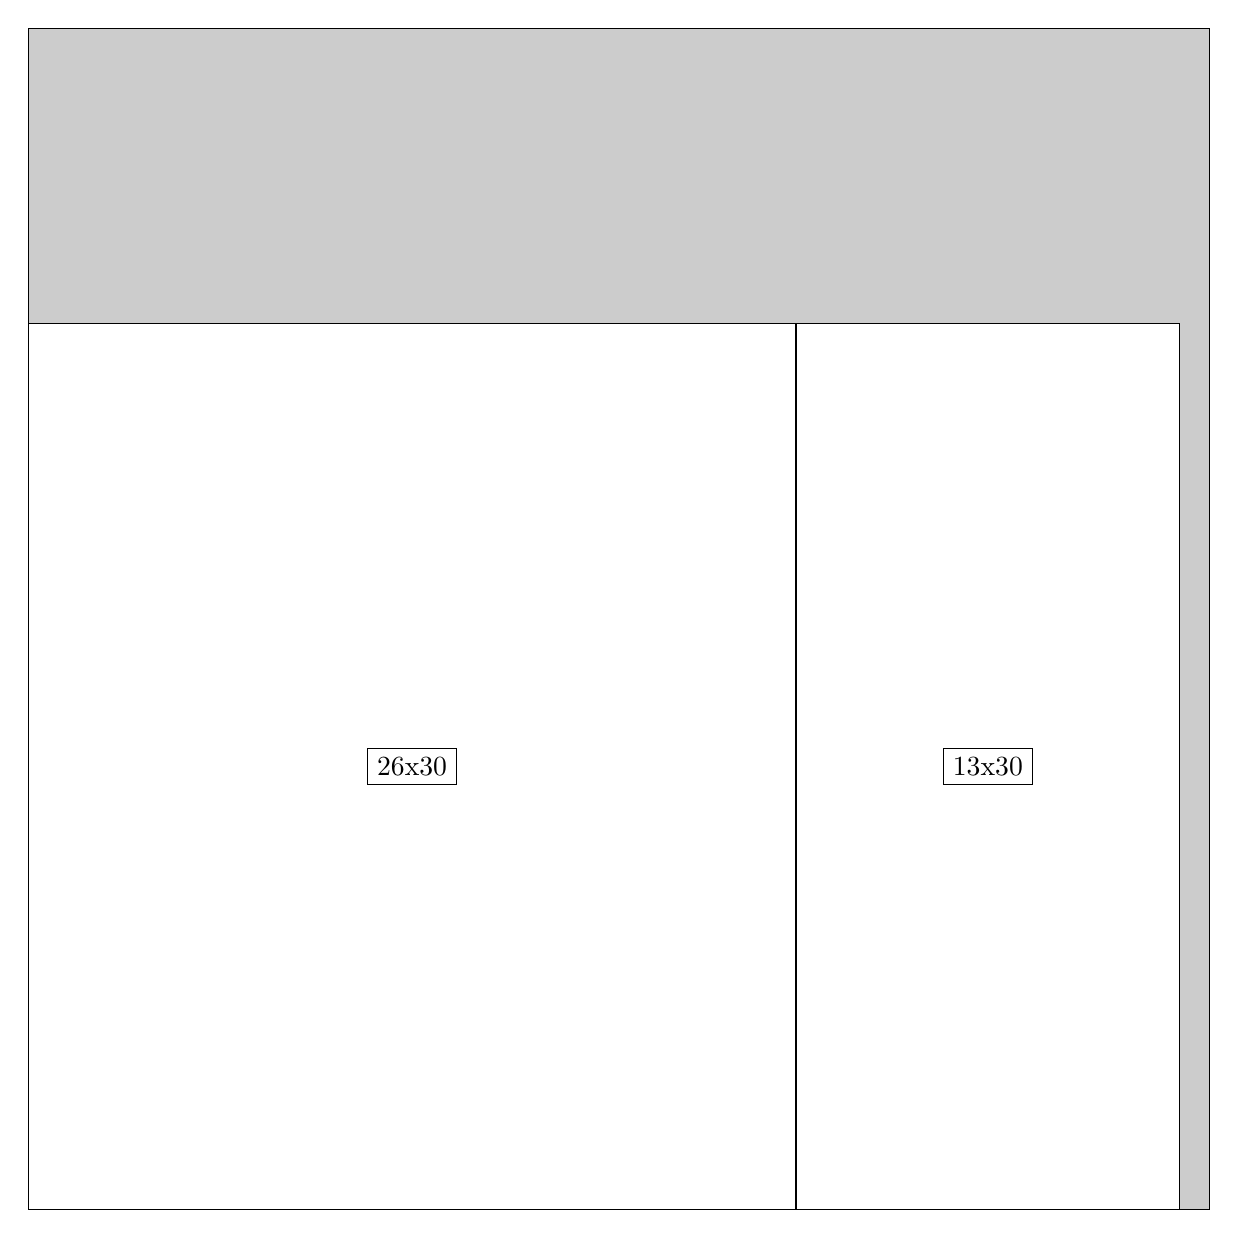
\begin{tikzpicture}[shorten >=1pt,scale=1.0,every node/.style={scale=1.0},->]
\tikzstyle{vertex}=[circle,fill=black!25,minimum size=14pt,inner sep=0pt]
\filldraw[fill=gray!40!white, draw=black] (0,0) rectangle (15.0,15.0);
\foreach \name/\x/\y/\w/\h in {26x30/0.0/0.0/9.75/11.25,13x30/9.75/0.0/4.875/11.25}
\filldraw[fill=white!40!white, draw=black] (\x,\y) rectangle node[draw] (\name) {\name} ++(\w,\h);
\end{tikzpicture}


w =26 , h =30 , x =0 , y =0 , v =780
\par
w =13 , h =30 , x =26 , y =0 , v =390
\par
\newpage


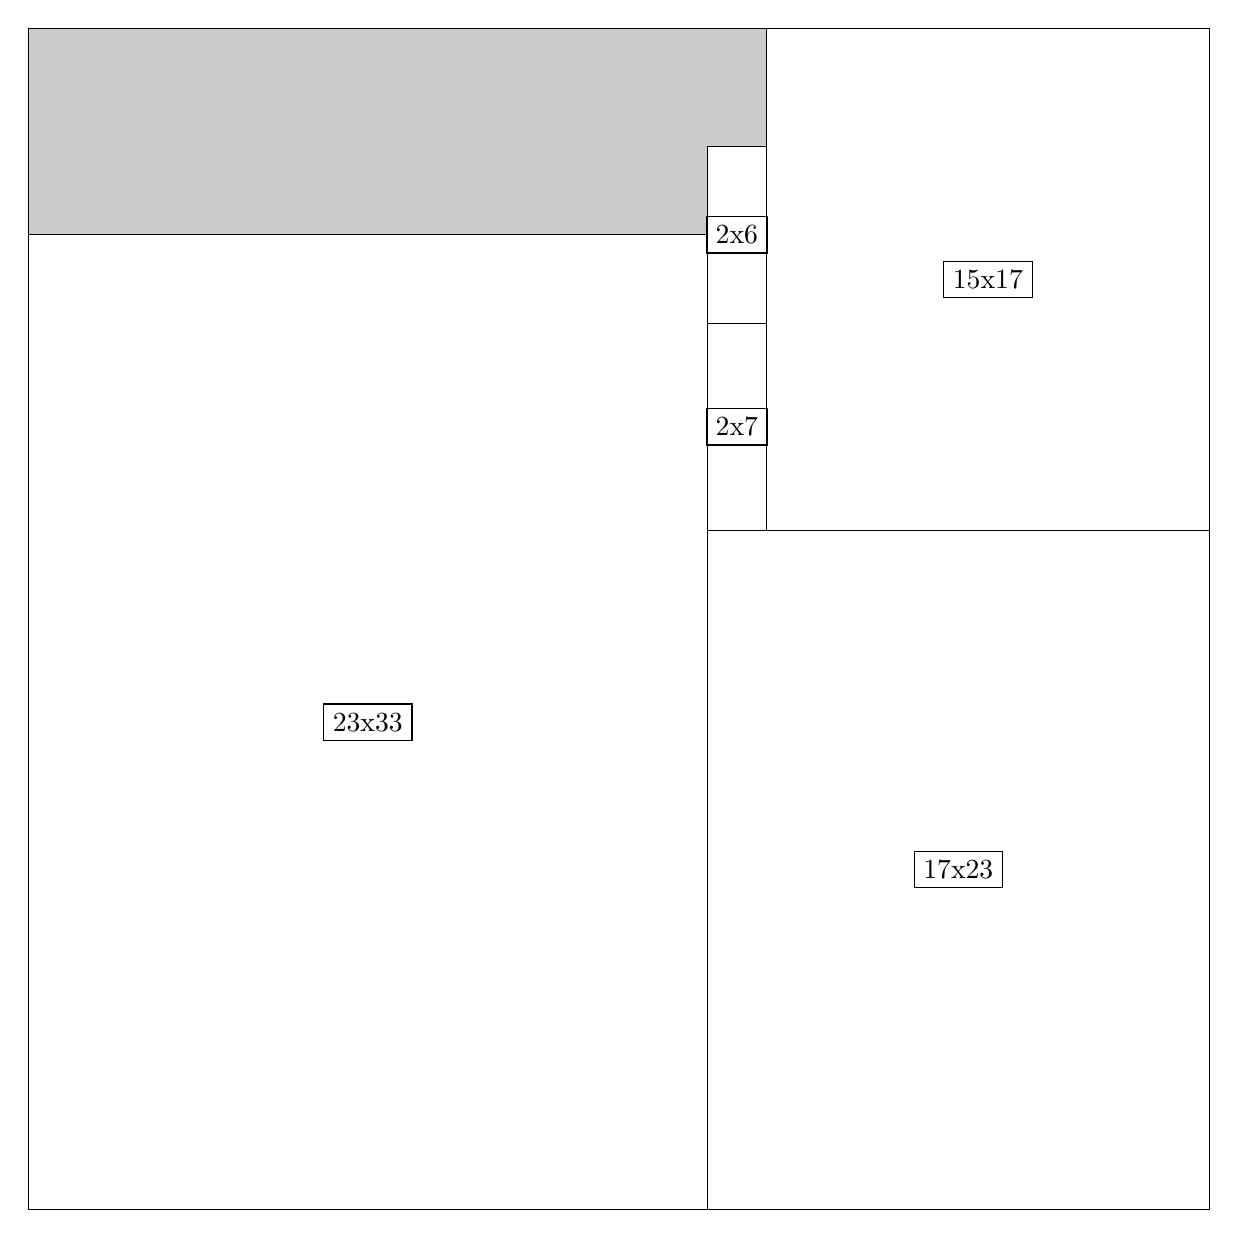
\begin{tikzpicture}[shorten >=1pt,scale=1.0,every node/.style={scale=1.0},->]
\tikzstyle{vertex}=[circle,fill=black!25,minimum size=14pt,inner sep=0pt]
\filldraw[fill=gray!40!white, draw=black] (0,0) rectangle (15.0,15.0);
\foreach \name/\x/\y/\w/\h in {23x33/0.0/0.0/8.625/12.375,17x23/8.625/0.0/6.375/8.625,15x17/9.375/8.625/5.625/6.375,2x7/8.625/8.625/0.75/2.625,2x6/8.625/11.25/0.75/2.25}
\filldraw[fill=white!40!white, draw=black] (\x,\y) rectangle node[draw] (\name) {\name} ++(\w,\h);
\end{tikzpicture}


w =23 , h =33 , x =0 , y =0 , v =759
\par
w =17 , h =23 , x =23 , y =0 , v =391
\par
w =15 , h =17 , x =25 , y =23 , v =255
\par
w =2 , h =7 , x =23 , y =23 , v =14
\par
w =2 , h =6 , x =23 , y =30 , v =12
\par
\newpage


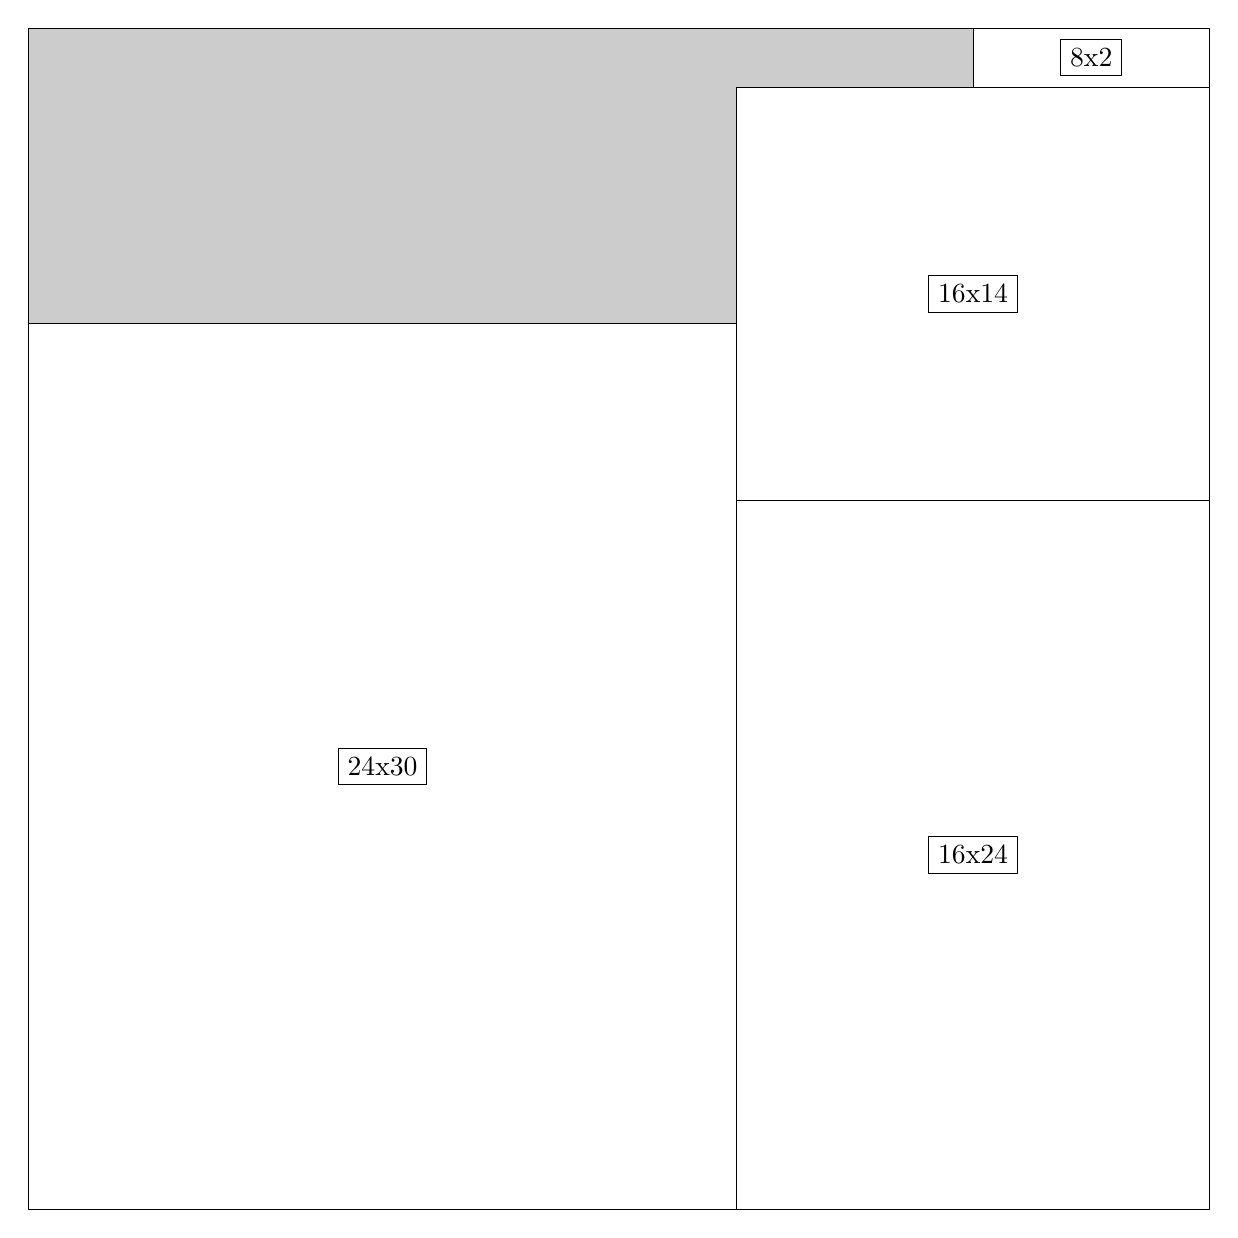
\begin{tikzpicture}[shorten >=1pt,scale=1.0,every node/.style={scale=1.0},->]
\tikzstyle{vertex}=[circle,fill=black!25,minimum size=14pt,inner sep=0pt]
\filldraw[fill=gray!40!white, draw=black] (0,0) rectangle (15.0,15.0);
\foreach \name/\x/\y/\w/\h in {24x30/0.0/0.0/9.0/11.25,16x24/9.0/0.0/6.0/9.0,16x14/9.0/9.0/6.0/5.25,8x2/12.0/14.25/3.0/0.75}
\filldraw[fill=white!40!white, draw=black] (\x,\y) rectangle node[draw] (\name) {\name} ++(\w,\h);
\end{tikzpicture}


w =24 , h =30 , x =0 , y =0 , v =720
\par
w =16 , h =24 , x =24 , y =0 , v =384
\par
w =16 , h =14 , x =24 , y =24 , v =224
\par
w =8 , h =2 , x =32 , y =38 , v =16
\par
\newpage


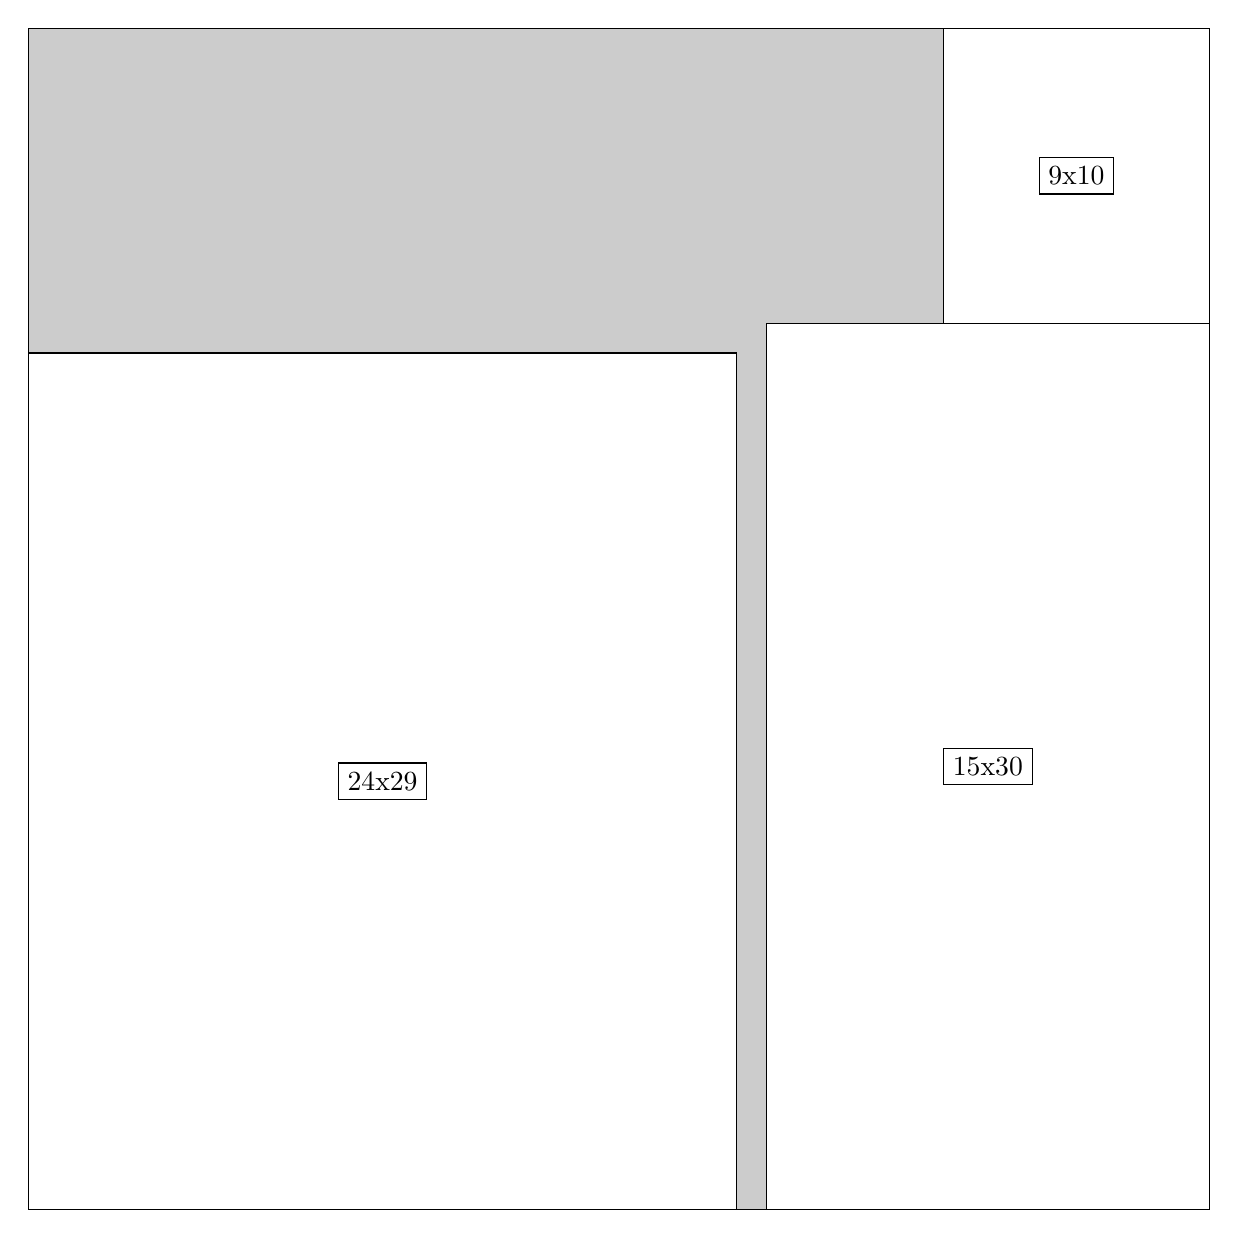
\begin{tikzpicture}[shorten >=1pt,scale=1.0,every node/.style={scale=1.0},->]
\tikzstyle{vertex}=[circle,fill=black!25,minimum size=14pt,inner sep=0pt]
\filldraw[fill=gray!40!white, draw=black] (0,0) rectangle (15.0,15.0);
\foreach \name/\x/\y/\w/\h in {24x29/0.0/0.0/9.0/10.875,15x30/9.375/0.0/5.625/11.25,9x10/11.625/11.25/3.375/3.75}
\filldraw[fill=white!40!white, draw=black] (\x,\y) rectangle node[draw] (\name) {\name} ++(\w,\h);
\end{tikzpicture}


w =24 , h =29 , x =0 , y =0 , v =696
\par
w =15 , h =30 , x =25 , y =0 , v =450
\par
w =9 , h =10 , x =31 , y =30 , v =90
\par
\newpage


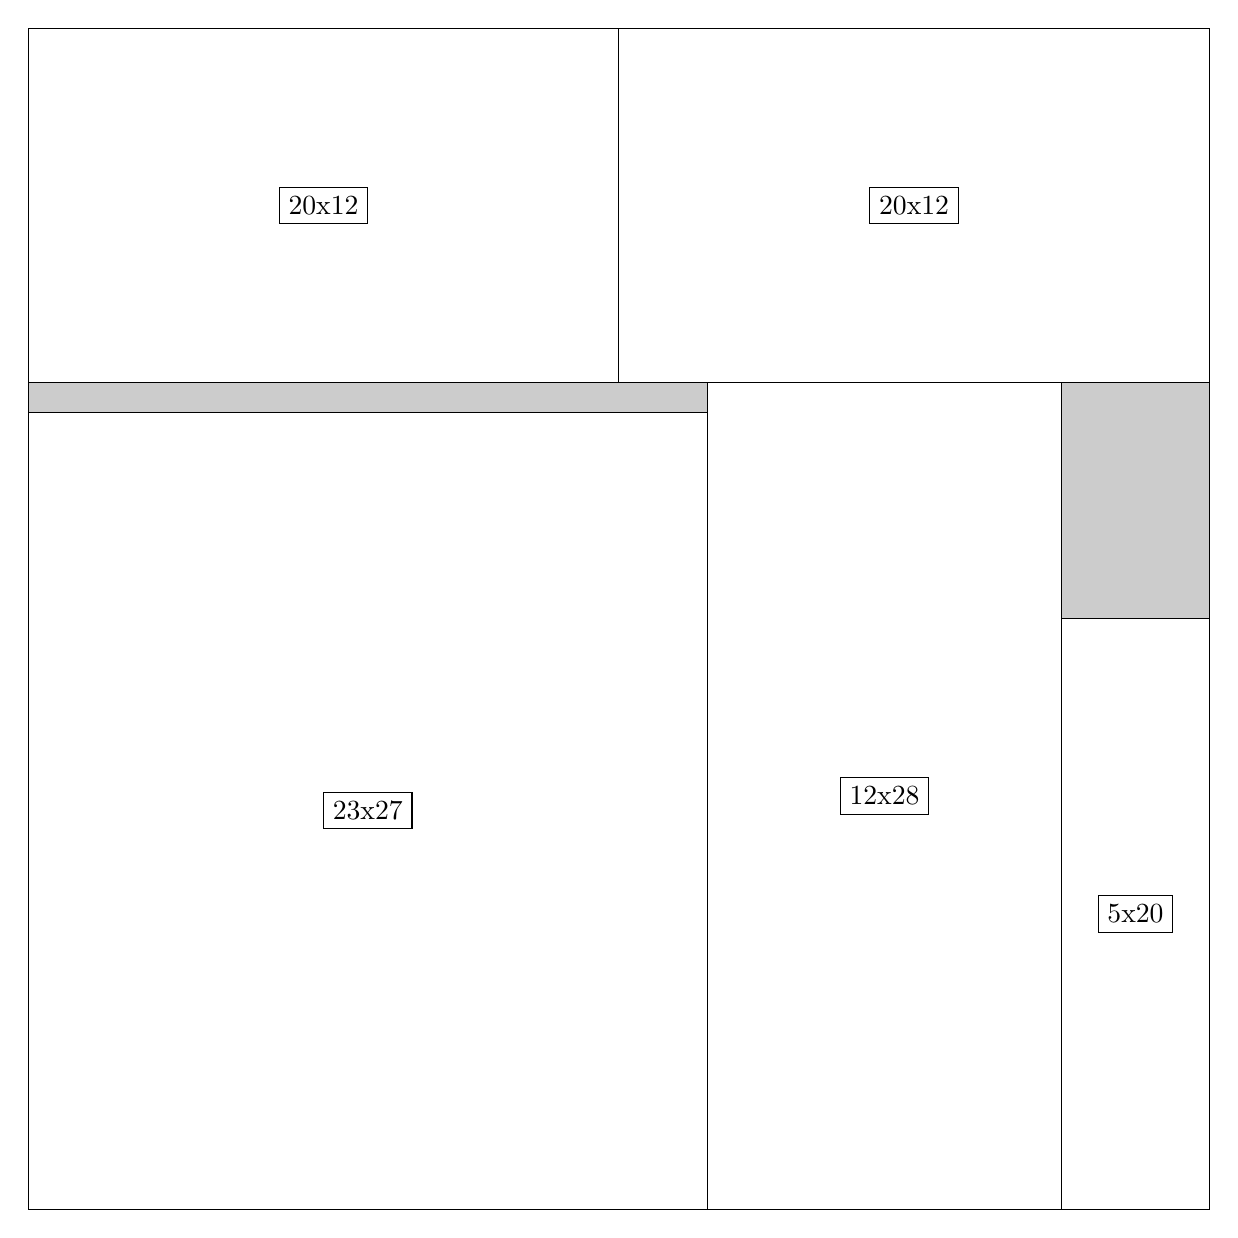
\begin{tikzpicture}[shorten >=1pt,scale=1.0,every node/.style={scale=1.0},->]
\tikzstyle{vertex}=[circle,fill=black!25,minimum size=14pt,inner sep=0pt]
\filldraw[fill=gray!40!white, draw=black] (0,0) rectangle (15.0,15.0);
\foreach \name/\x/\y/\w/\h in {23x27/0.0/0.0/8.625/10.125,12x28/8.625/0.0/4.5/10.5,20x12/0.0/10.5/7.5/4.5,20x12/7.5/10.5/7.5/4.5,5x20/13.125/0.0/1.875/7.5}
\filldraw[fill=white!40!white, draw=black] (\x,\y) rectangle node[draw] (\name) {\name} ++(\w,\h);
\end{tikzpicture}


w =23 , h =27 , x =0 , y =0 , v =621
\par
w =12 , h =28 , x =23 , y =0 , v =336
\par
w =20 , h =12 , x =0 , y =28 , v =240
\par
w =20 , h =12 , x =20 , y =28 , v =240
\par
w =5 , h =20 , x =35 , y =0 , v =100
\par
\newpage


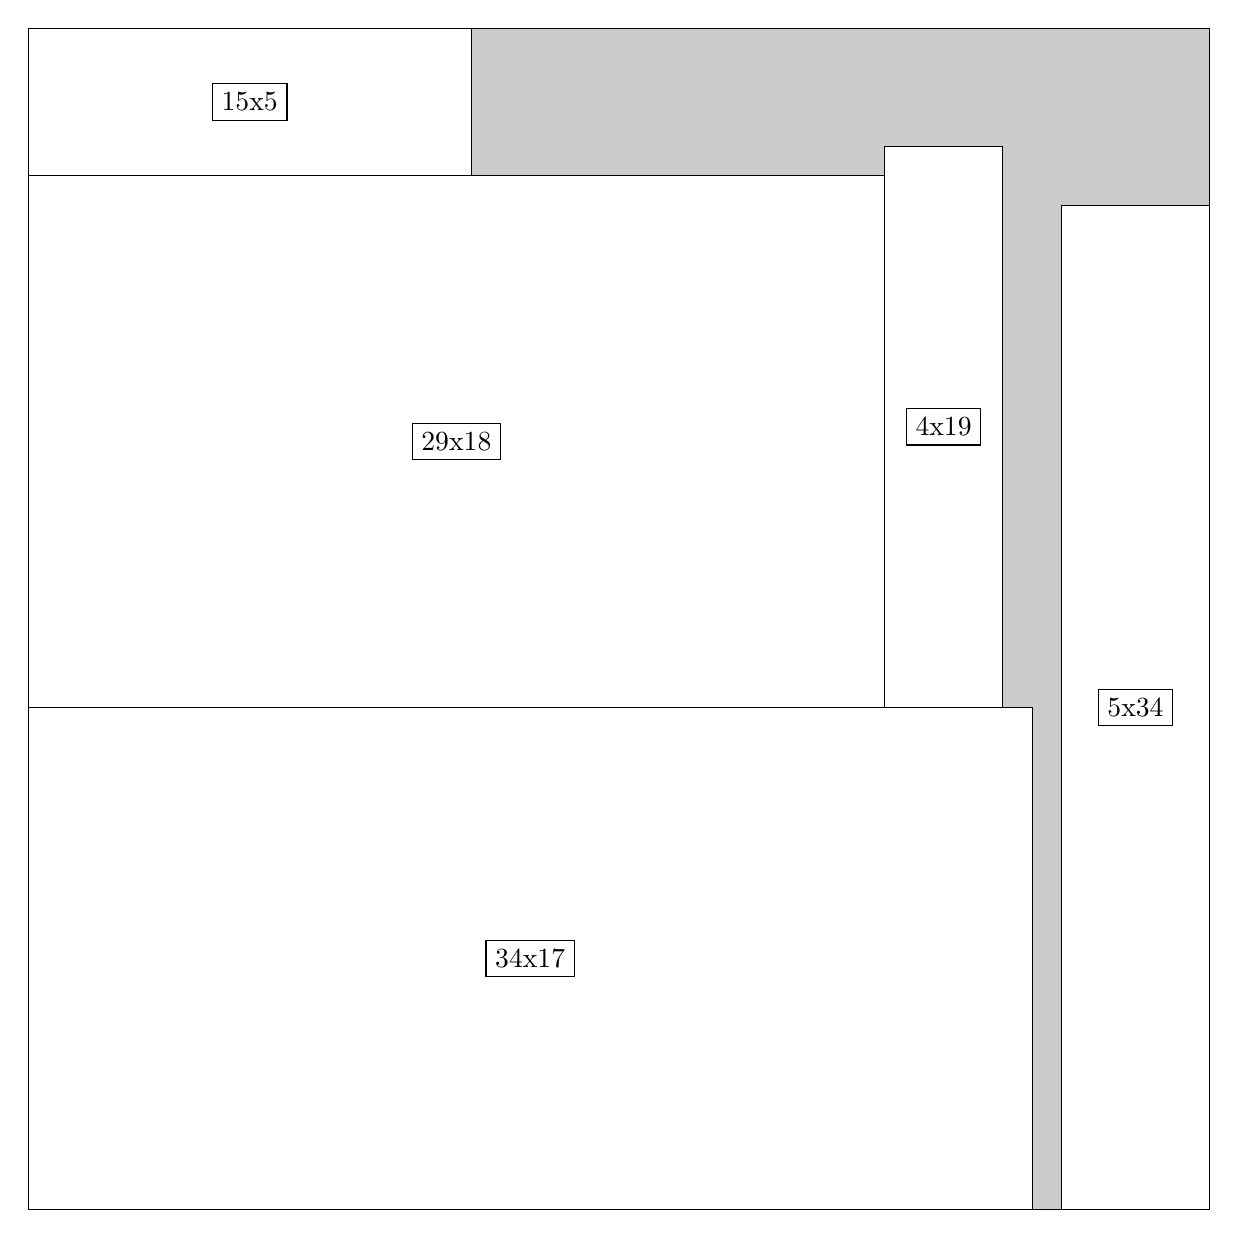
\begin{tikzpicture}[shorten >=1pt,scale=1.0,every node/.style={scale=1.0},->]
\tikzstyle{vertex}=[circle,fill=black!25,minimum size=14pt,inner sep=0pt]
\filldraw[fill=gray!40!white, draw=black] (0,0) rectangle (15.0,15.0);
\foreach \name/\x/\y/\w/\h in {34x17/0.0/0.0/12.75/6.375,29x18/0.0/6.375/10.875/6.75,15x5/0.0/13.125/5.625/1.875,5x34/13.125/0.0/1.875/12.75,4x19/10.875/6.375/1.5/7.125}
\filldraw[fill=white!40!white, draw=black] (\x,\y) rectangle node[draw] (\name) {\name} ++(\w,\h);
\end{tikzpicture}


w =34 , h =17 , x =0 , y =0 , v =578
\par
w =29 , h =18 , x =0 , y =17 , v =522
\par
w =15 , h =5 , x =0 , y =35 , v =75
\par
w =5 , h =34 , x =35 , y =0 , v =170
\par
w =4 , h =19 , x =29 , y =17 , v =76
\par
\newpage


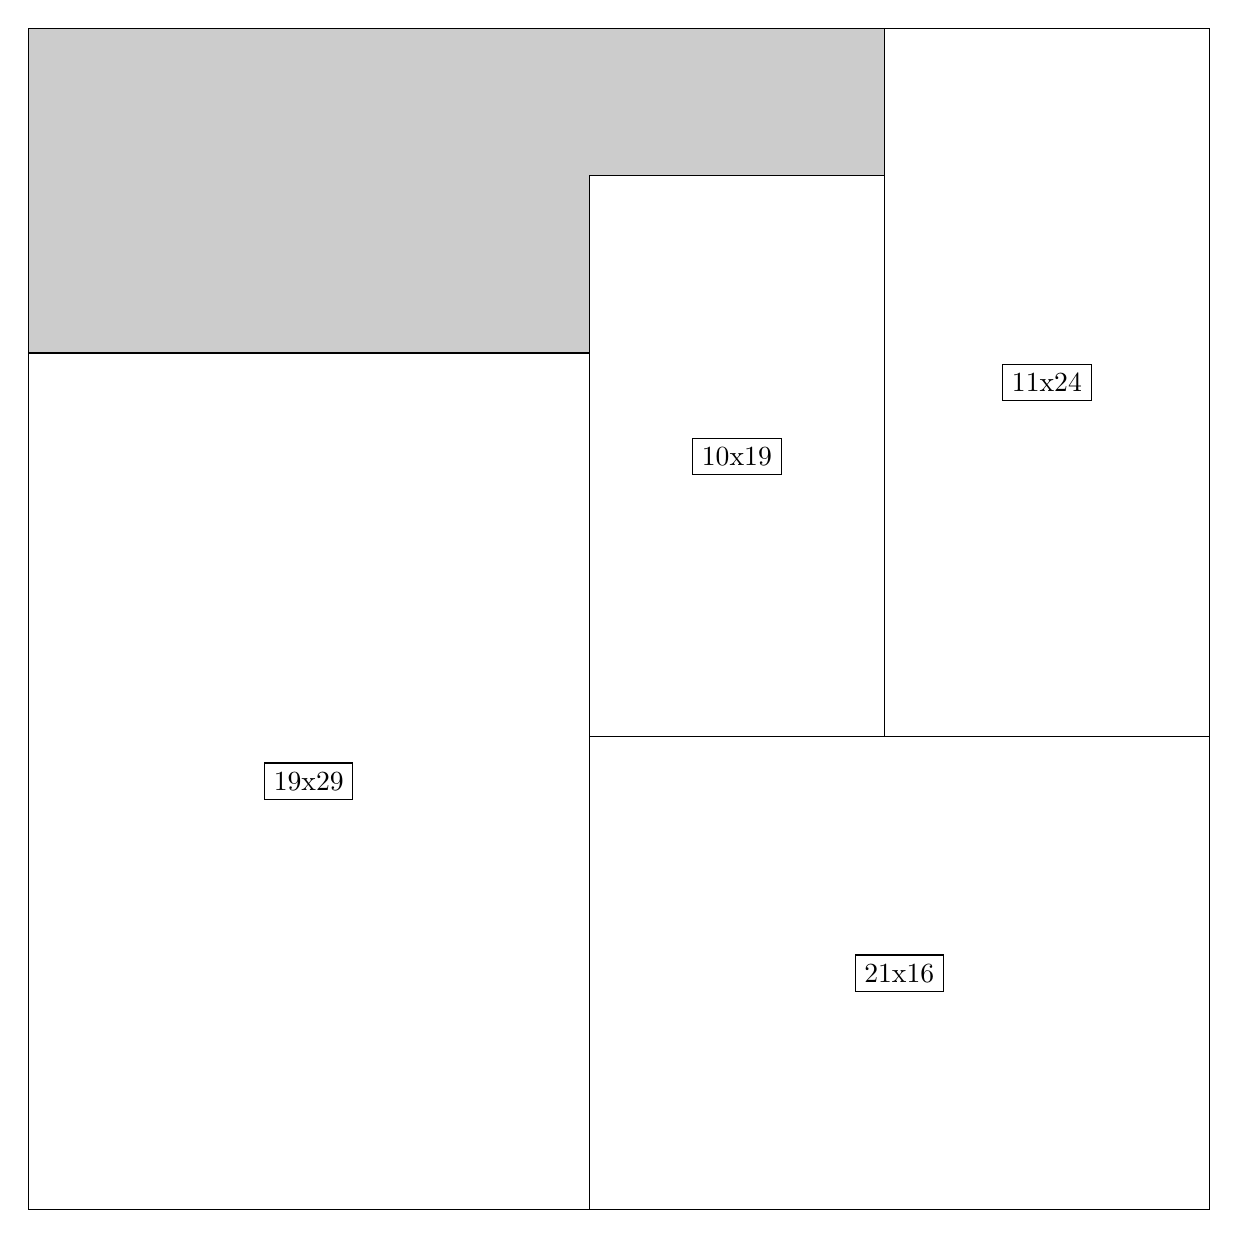
\begin{tikzpicture}[shorten >=1pt,scale=1.0,every node/.style={scale=1.0},->]
\tikzstyle{vertex}=[circle,fill=black!25,minimum size=14pt,inner sep=0pt]
\filldraw[fill=gray!40!white, draw=black] (0,0) rectangle (15.0,15.0);
\foreach \name/\x/\y/\w/\h in {19x29/0.0/0.0/7.125/10.875,11x24/10.875/6.0/4.125/9.0,10x19/7.125/6.0/3.75/7.125,21x16/7.125/0.0/7.875/6.0}
\filldraw[fill=white!40!white, draw=black] (\x,\y) rectangle node[draw] (\name) {\name} ++(\w,\h);
\end{tikzpicture}


w =19 , h =29 , x =0 , y =0 , v =551
\par
w =11 , h =24 , x =29 , y =16 , v =264
\par
w =10 , h =19 , x =19 , y =16 , v =190
\par
w =21 , h =16 , x =19 , y =0 , v =336
\par
\newpage


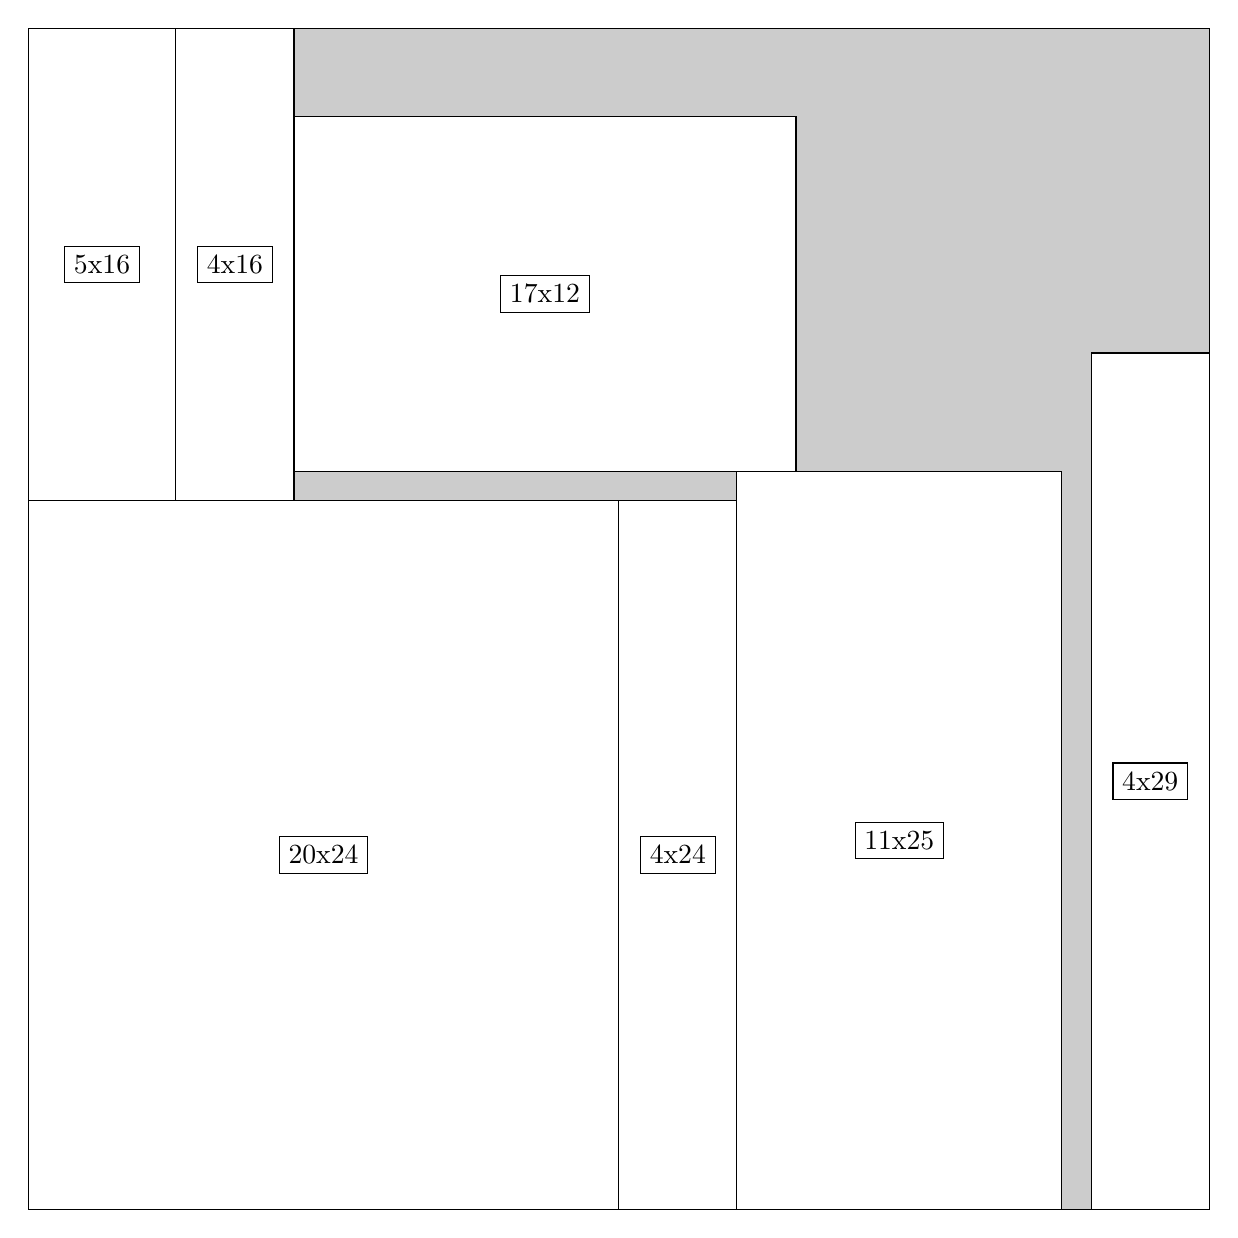
\begin{tikzpicture}[shorten >=1pt,scale=1.0,every node/.style={scale=1.0},->]
\tikzstyle{vertex}=[circle,fill=black!25,minimum size=14pt,inner sep=0pt]
\filldraw[fill=gray!40!white, draw=black] (0,0) rectangle (15.0,15.0);
\foreach \name/\x/\y/\w/\h in {20x24/0.0/0.0/7.5/9.0,11x25/9.0/0.0/4.125/9.375,17x12/3.375/9.375/6.375/4.5,4x24/7.5/0.0/1.5/9.0,4x29/13.5/0.0/1.5/10.875,5x16/0.0/9.0/1.875/6.0,4x16/1.875/9.0/1.5/6.0}
\filldraw[fill=white!40!white, draw=black] (\x,\y) rectangle node[draw] (\name) {\name} ++(\w,\h);
\end{tikzpicture}


w =20 , h =24 , x =0 , y =0 , v =480
\par
w =11 , h =25 , x =24 , y =0 , v =275
\par
w =17 , h =12 , x =9 , y =25 , v =204
\par
w =4 , h =24 , x =20 , y =0 , v =96
\par
w =4 , h =29 , x =36 , y =0 , v =116
\par
w =5 , h =16 , x =0 , y =24 , v =80
\par
w =4 , h =16 , x =5 , y =24 , v =64
\par
\newpage


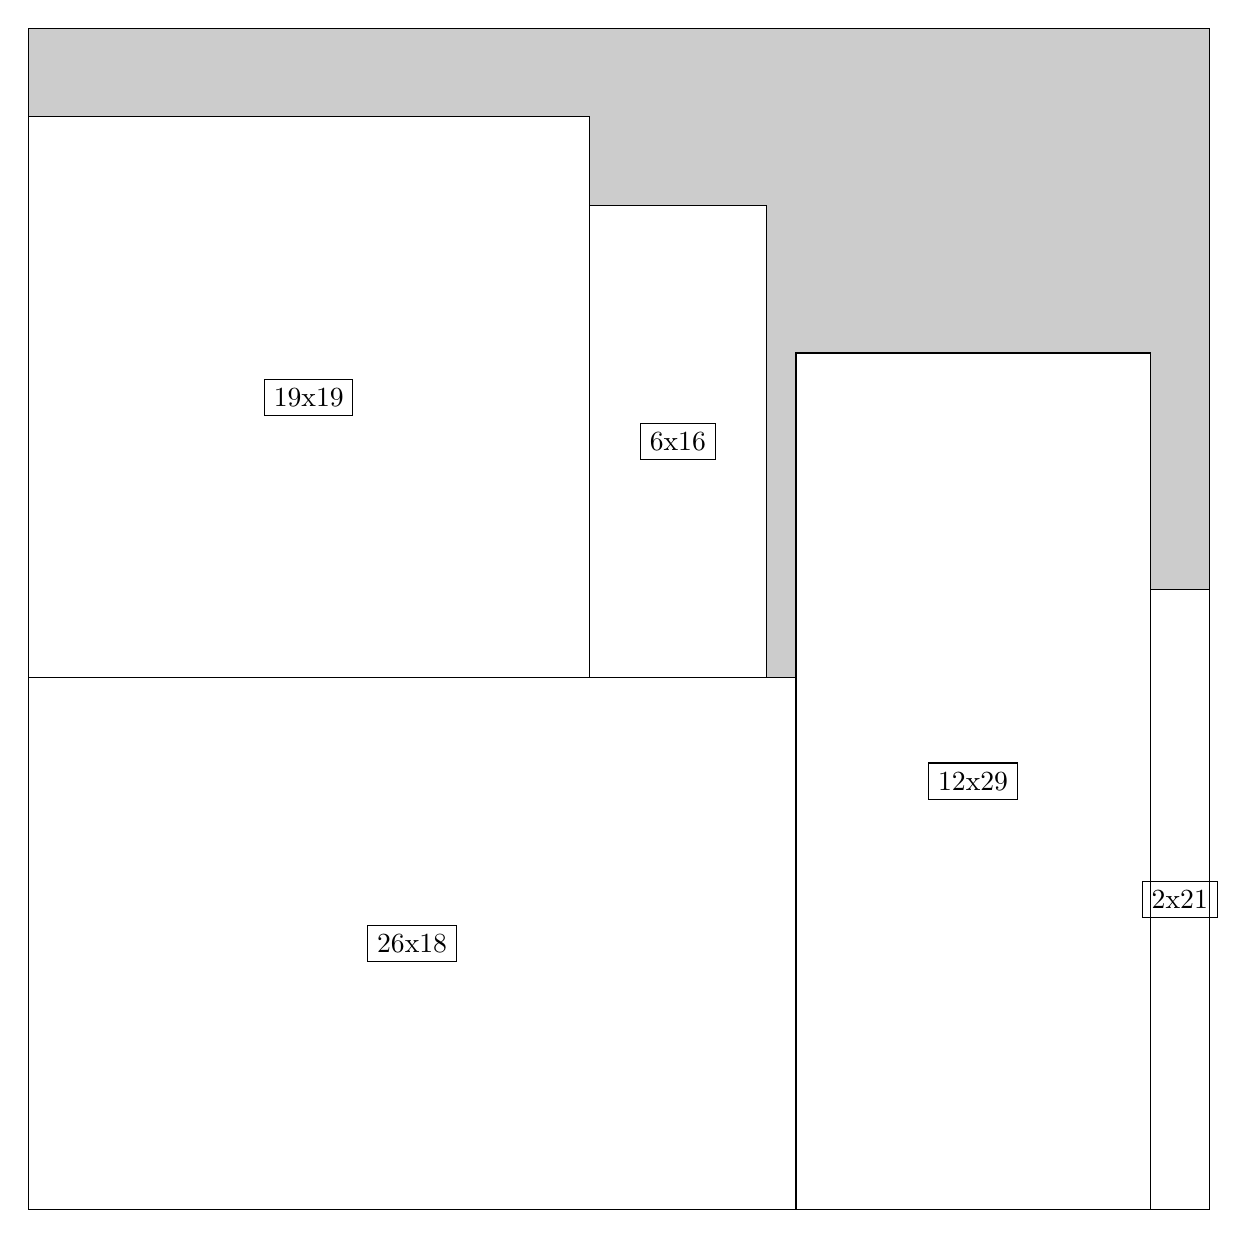
\begin{tikzpicture}[shorten >=1pt,scale=1.0,every node/.style={scale=1.0},->]
\tikzstyle{vertex}=[circle,fill=black!25,minimum size=14pt,inner sep=0pt]
\filldraw[fill=gray!40!white, draw=black] (0,0) rectangle (15.0,15.0);
\foreach \name/\x/\y/\w/\h in {26x18/0.0/0.0/9.75/6.75,19x19/0.0/6.75/7.125/7.125,12x29/9.75/0.0/4.5/10.875,6x16/7.125/6.75/2.25/6.0,2x21/14.25/0.0/0.75/7.875}
\filldraw[fill=white!40!white, draw=black] (\x,\y) rectangle node[draw] (\name) {\name} ++(\w,\h);
\end{tikzpicture}


w =26 , h =18 , x =0 , y =0 , v =468
\par
w =19 , h =19 , x =0 , y =18 , v =361
\par
w =12 , h =29 , x =26 , y =0 , v =348
\par
w =6 , h =16 , x =19 , y =18 , v =96
\par
w =2 , h =21 , x =38 , y =0 , v =42
\par
\newpage


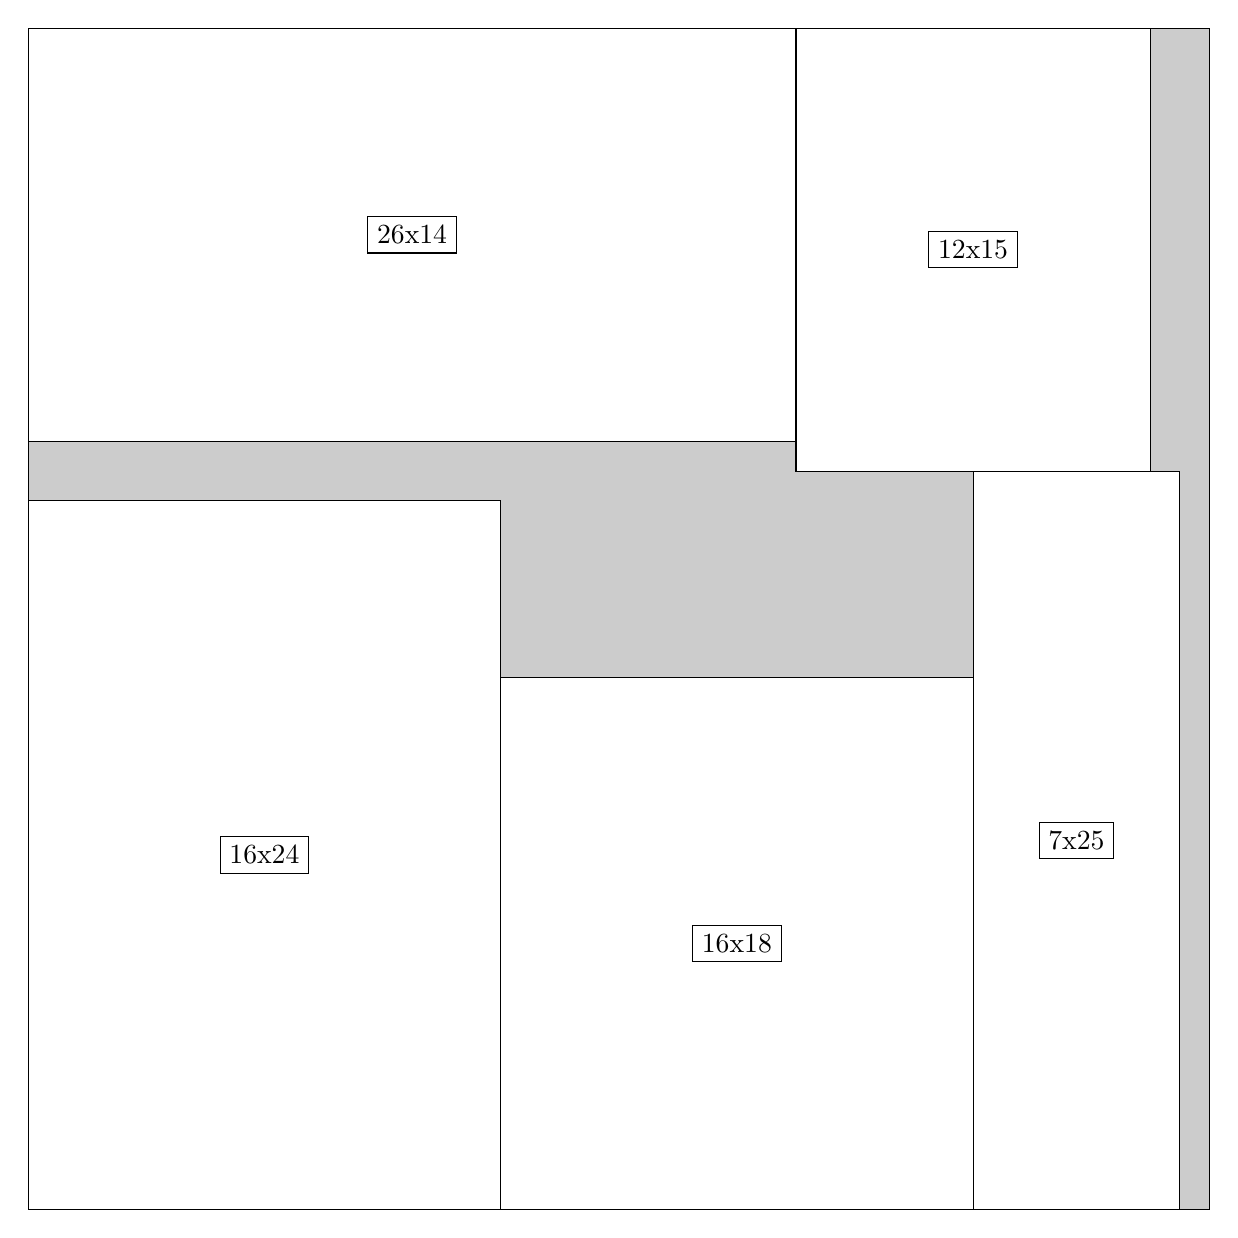
\begin{tikzpicture}[shorten >=1pt,scale=1.0,every node/.style={scale=1.0},->]
\tikzstyle{vertex}=[circle,fill=black!25,minimum size=14pt,inner sep=0pt]
\filldraw[fill=gray!40!white, draw=black] (0,0) rectangle (15.0,15.0);
\foreach \name/\x/\y/\w/\h in {16x24/0.0/0.0/6.0/9.0,26x14/0.0/9.75/9.75/5.25,16x18/6.0/0.0/6.0/6.75,12x15/9.75/9.375/4.5/5.625,7x25/12.0/0.0/2.625/9.375}
\filldraw[fill=white!40!white, draw=black] (\x,\y) rectangle node[draw] (\name) {\name} ++(\w,\h);
\end{tikzpicture}


w =16 , h =24 , x =0 , y =0 , v =384
\par
w =26 , h =14 , x =0 , y =26 , v =364
\par
w =16 , h =18 , x =16 , y =0 , v =288
\par
w =12 , h =15 , x =26 , y =25 , v =180
\par
w =7 , h =25 , x =32 , y =0 , v =175
\par
\newpage


\end{document}